\documentclass[10pt,a4paper]{beamer}
\usepackage{amsmath, amssymb, mathtools}
\usepackage{amsthm}
\usepackage{fontspec}
\usepackage{xunicode}
\usepackage{fancyhdr}
\usepackage[french]{babel}
\usepackage{algorithm, algorithmic}
\usepackage{listings}
\usepackage{graphicx}


\usetheme{Darmstadt}
\setbeamertemplate{navigation symbols}{}
\setbeamertemplate{blocks}[]
\usefonttheme[onlymath]{serif}

\institute{Sorbonne Université}
\title[Center text]{\textbf{Composition modulaire des polynômes à une variable}}
\subtitle{\small{Encadrant : M. Vincent NEIGER}}
\author{Serigne Fallou FALL \and Marie BONBOIRE}
\date{}


\begin{document}

\begin{frame}[plain]
    \titlepage
\end{frame}


\section{Introduction}
\begin{frame}
    \tableofcontents[currentsection]
\end{frame}

\begin{frame}
    Environnement :
    \begin{itemize}
        \item Corps d'étude : $\mathbb{Z}/p\mathbb{Z} := {k | k\in{0, ..., p-1}}$
        \item Implantation : Sagemath (Python) et NTL (C++)  
    \end{itemize}

    Notions primaires :
    \begin{itemize}
        \item addition, soustraction, division euclidienne
    \end{itemize}
\end{frame}

%%%%%%%%%%%%%%%%%%%%%%%%%%%%%%%%%%%%%%%%
\section{Multiplication}
\begin{frame}
    \tableofcontents[currentsection]
\end{frame}

\begin{frame}
    \begin{block}{Multiplication de polynômes}
        \textbf{Require :} $f,g \in \mathbb{Z}/p\mathbb{Z}[x]$ de degré au plus $n-1$ \\
        \textbf{Ensure :} $f*g$
    \end{block}
    \rule{\linewidth}{0.2mm}\\[0.5cm]
    \textbf{Algorithme naïf}
    \[
    f*g=\sum_{i=0}^{2n-2} (\sum_{j+k=i}f_j*g_k) x^i
    \]

    \begin{alertblock}{Complexité}
        L'algorithme naïf est en $O(n^2)$
    \end{alertblock}

\end{frame}

\begin{frame}
    \textbf{Algorithme de Karatsuba}
    \begin{align*}
        f*g &= F^{(0)}G^{(0)}\\
            &+\left((F^{(0)}+F^{(1)}) (G^{(0)} + G^{(1)}) - F^{(0)}G^{(0)} - F^{(1)}G^{(1)}\right)x^k\\
            &+F^{(1)}G^{(1)}x^{2k} 
    \end{align*}

    \begin{alertblock}{Complexité}
        L'algorithme de Karatsuba est en $O(n^{log_2(3)})$
    \end{alertblock}
    \rule{\linewidth}{0.2mm}\\[0.5cm]
    [comparaisons complexité]
    
\end{frame}


%%%%%%%%%%%%%%%%%%%%%%%%%%%%%%%%%%%%%%%%
\section{Composition modulaire des polynômes à une variable}
\begin{frame}
    \tableofcontents[currentsection]
\end{frame}

\begin{frame}
    \begin{block}{Composition modulaire}
        \textbf{Require :} $f \in \mathbb{Z}/p\mathbb{Z}[x]$ de degré n, $a \in \mathbb{Z}/p\mathbb{Z}[x]$ de degré au plus $n-1$, $g \in \mathbb{Z}/p\mathbb{Z}[y]$ de degré au plus $d$. \\
        \textbf{Ensure :} $g(a) \% f$
    \end{block}
    \rule{\linewidth}{0.2mm}\\[0.5cm]
    
    \textbf{Algorithme naïf et Horner}
    \begin{align*}
        g(a)\%f &=(g_0+g_1a+g_2a^2+...+g_na^n) \%f \\
            &=(...((g_{n}a \%f +g_{n-1})a \%f+g_{n-2})...)a \%f+g_0 \%f    
    \end{align*}

    \begin{alertblock}{Complexité}
        L'algorithme naïf est en $O(?)$ (quadratique) tandis que l'algorithme d'Horner est en $O(?)$ (linéaire)
    \end{alertblock}
\end{frame}

\begin{frame}
    \textbf{Algorithme de Brent et Kung}
    \begin{itemize}
        \item Choix de r et s : $r = \lceil \sqrt{d} \rceil$, $s = \lceil d/r \rceil$ 
        \item Calcul simultané d
            \[
            \begin{pmatrix}
                g_0&g_1&...&g_{r-1} \\
                g_r&g_{r+1}&...&g_{2r-1} \\
                \vdots&\vdots&...&\vdots \\
                g_{}&g_{}&...&g_{r^2-1}
            \end{pmatrix}
            \begin{pmatrix}
                1 \\
                a \\
                a^2 \\
                ... \\
                a^r
            \end{pmatrix}
            \]
        \item Retourne l'évaluation d'horner des b
    \end{itemize}

    \begin{alertblock}{Complexité}
        L'algorithme de Brent et Kung est en $O((1+n/d)d^{\omega_2/2})$
    \end{alertblock}
\end{frame}

\begin{frame}
    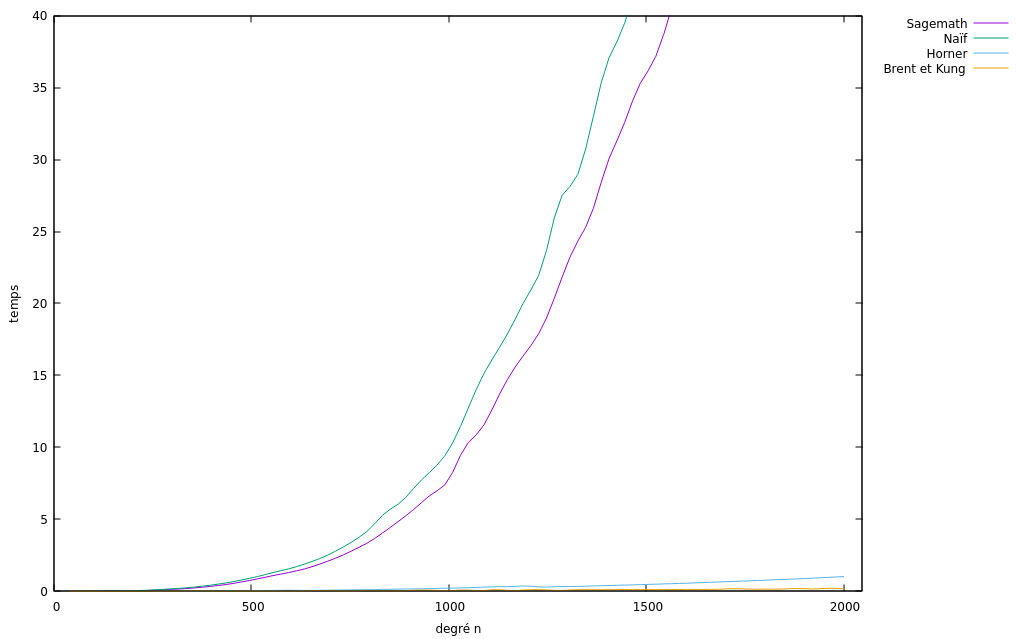
\includegraphics[width=1\linewidth]{comp.png}
\end{frame}

%%%%%%%%%%%%%%%%%%%%%%%%%%%%%%%%%%%%%%%%%%ù
\section{Algorithme de Nusken et Ziegler}
\begin{frame}
    \tableofcontents[currentsection]
\end{frame}

\begin{frame}    
    \begin{block}{Nusken et Ziegler}
        \textbf{Require :} $f \in \mathbb{Z}/p\mathbb{Z}[X]$ de degré n, $a \in \mathbb{Z}/p\mathbb{Z}[X]$ de degré au plus $n-1$, $g \in \mathbb{Z}/p\mathbb{Z}[x,y]$ de degré au plus $d$. \\
        \textbf{Ensure :} g(a) \% f
    \end{block}

    \[
    g(x,y) = \sum_{i,j<\delta}g_{i+\delta j}(x)y^{i+\delta j} = \sum_{j<\delta} \left( \sum_{i<\delta} g_{i+\delta j}(x)y^i \right) y^{\delta j}     
    \]

    \begin{itemize}
        \item Calcul simultané des $R_j = g_{i+\delta j}(x)a^i \%f $
            \[
            \begin{pmatrix}
                R_0 \\
                R_1 \\
                \vdots \\
                R_{\delta-1}
            \end{pmatrix}
            =
            \begin{pmatrix}
                g_0(x)&g_1(x)&...&g_{\delta -1}(x) \\
                g_{\delta}(x)&g_{1+\delta}(x)&...&g_{2\delta-1}(x) \\
                \vdots&\vdots&...&\vdots \\
                g_{(\delta-1)\delta}(x)&g_{(\delta-1)\delta+1}(x)&...&g_{\delta^2-1}(x)
            \end{pmatrix}
            \begin{pmatrix}
                1 \\
                a \\
                a^2 \%f \\
                ... \\
                a^{\delta-1} \%f
            \end{pmatrix}
            \]
        \item Pour $j\in{0,...,\delta-1}$, $a_j=a^{\delta j}\% f$
        \item Retourne $\sum_{j<\delta}(R_ja_j \% f)$
    \end{itemize}

    
\end{frame}

\begin{frame}
    \begin{alertblock}{Complexité}
        L'algorithme de Nusken et Ziegler est en $O(d_yM(d_x) + d_yM(n))$
    \end{alertblock}
\end{frame}

\section{Conclusion}
\begin{frame}
    \tableofcontents[currentsection]
\end{frame}


\end{document}
